
\begin{figure}
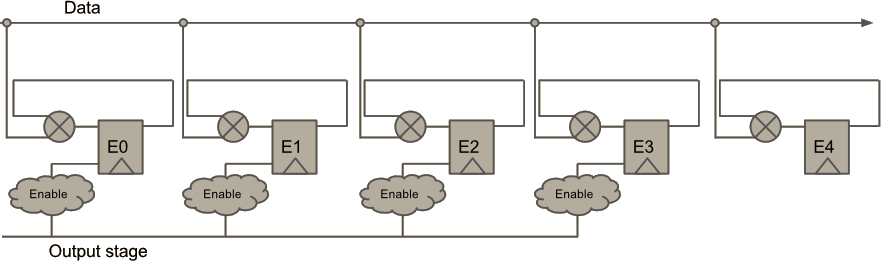
\includegraphics[width=15cm]{implementation/fig_ecc}
\caption{Implementation of Hamming(16,11)}
\label{fig:ecc}
\end{figure}

In this section, we describe how the module designs detailed in
\autoref{sec:design} are implemented on a Xilinx Virtex4
XC4VFX12-SF363-12 FPGA. The modules are not represented as separate
VHDL files or entities , but are only a conceptual model of how the
system works.

\subsection{Technology Schematic}
\label{sec:technologyschematic}

Figure \autoref{fig:technologyschematic} shows how each functionality
of the Liaison from \autoref{fig:overview} is mapped to the LUTs in
the syntesised design.  Each functionality are marked with a distinct
colour. Note that LUTs marked as either ``Status Calculation'' or
``State Maintenance'' functionality are both a part of the State
Maintenance module.


\begin{figure}[p]
  \vspace*{-1.2in}
  \centerline{ 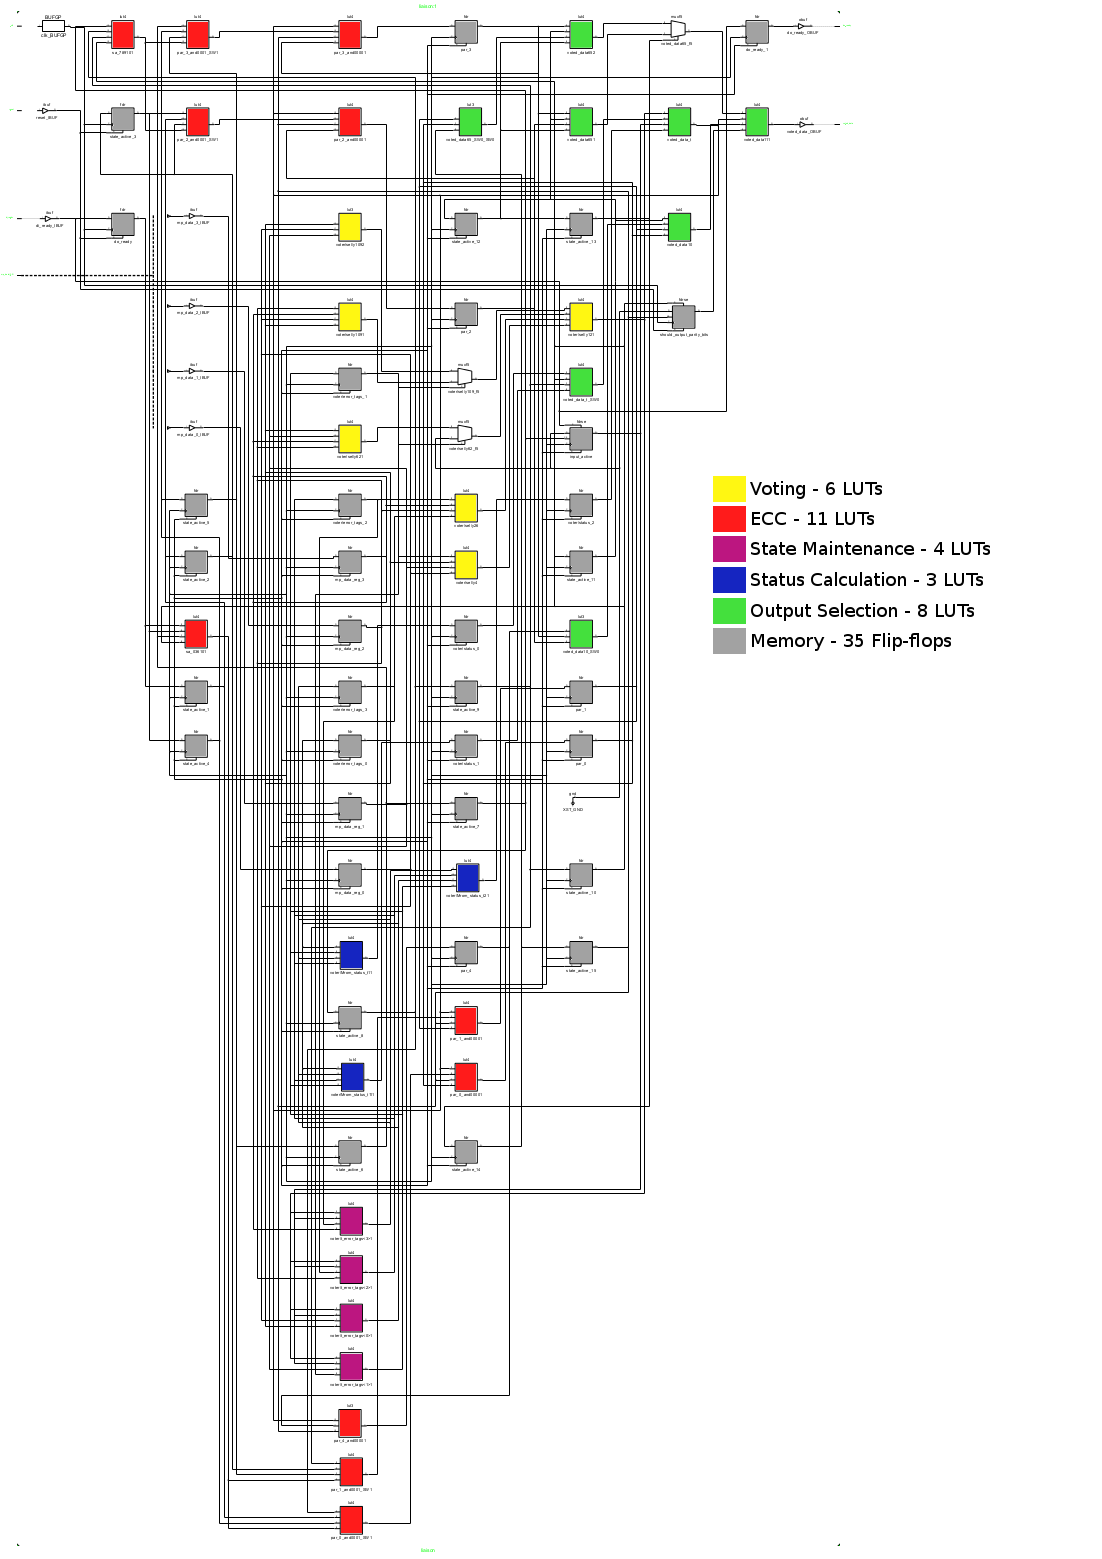
\includegraphics[width=1.2\textwidth]{LUT-count} }
  \caption{The technology schematic of our Liaison}
  \label{fig:technologyschematic}
\end{figure}

\subsection{Voting Algorithm Implementation}
The implementation of our voting algorithm, described in
\autoref{sec:votingalgorithm}, consists of six LUTs and two MUXes. The 

%NO NO NO red.anm.
%It is impossible for man to figure out what the hell these LUTs
%do... they certainly do not match the VHDL code.

\subsection{State Maintenance Implementation}
The state maintenance is implemented with the required number of
registers. 

Since we send 16 bits per voted word, the output stage
state is represented by 16 flip-flops connected in sequence,
implementing a shift-register. 

The error tags are implemented with four flip-flops. To update the
error tags, one LUT is used to calculate the new value of each flip
flop. These LUTs take as input the old error tag value, the
microcontroller data, the result of the vote and the enable signal. If
the old error tag was set, the new error tag is also set. Else, if the
enable signal is high, the error tag is set if the microcontroller
data differs from the voted data.

The status bits are calculated based on the error tags. Since there
are only four error tags, we can calculate each status bit with one
LUT each, so the status calculation is implemented with 3 LUTs. 

The state also includes five parity bit registers, whose update
semantics will be explained in in \autoref{sec:eccimplementation}.

\subsection{Error Correction Code Implementation}
\label{sec:eccimplementation}
Apart from the SECDED bit, each parity bit calculates the parity over
some subset of data bits. Since the data is computed sequentially and
the parity bits are computed on the fly as the data is being sent, it
is necessary to implement some control logic for each parity bit to
determine whether the current data bit being sent is one the parity
bit is supposed to cover or not. 

Since the equations 

For the SECDEC bit, only one LUT is necessary, since the 

Since the ECC is computed on the fly, 

The error code calculation uses most of its LUTs on calculating the
signals

\subsection{Output Selection Implementation}

\subsection{Results}

\todo[inline]{Describe LUT usage, register usage and clock frequency}
